\chapter{Study 1: Does the Meeting Loss Save Compute?}\label{ch:study1}

This chapter answers RQ1. It first reports how the arms were selected (\cref{sec:selection}), then the pre-registered test (\cref{sec:h1}), then the controls and variants (\cref{sec:desc}), the gradient alignment (\cref{sec:h3}), and finally the finding about tuning noise that this study produced (\cref{sec:noise}).

\section{Selection stage}\label{sec:selection}
Every arm was tuned with the 25-trial search of \cref{sec:tuning}; \cref{tab:selection} lists the best trial of each arm and the median of its 25 trials (\tierE{}, selection seeds 1000 and 1001 for the first tuning). At this stage, no variant of the meeting loss beat the tuned baseline: D was $19\%$ worse than A in the selection score, and the frozen-inverse variant V3 was about level with A ($225.1$ against $232.6$) while having almost no alignment with the task gradient. Deep supervision (B) was $18\%$ \emph{better} than A at the selection level ($191.2$ against $232.6$ GFLOPs), which turned out not to survive fresh seeds (\cref{sec:h1}). The second tuning of the baseline (A2) tied with A1 exactly at selection ($232.6$).

\begin{table}[t]
\centering\small
\caption{Selection stage. Best trial of each arm (2 selection seeds, mean GFLOPs to $0.975$) and the median over its 25 trials. ``Late accuracy'' is the mean validation accuracy over the last five evaluations of the winning trial.}
\label{tab:selection}
\begin{tabular}{@{}l r r r@{}}
\toprule
Arm & Best GFLOPs to 0.975 & Median of 25 trials & Late accuracy\\
\midrule
A (= A1) & 232.6 & 383.8 & 0.9802 \\
A2 (re-tuning) & 232.6 & 368.3 & 0.9802 \\
B & 191.2 & 429.1 & 0.9813 \\
B-code & 230.2 & 468.1 & 0.9812 \\
C & 418.0 & 810.8 & 0.9812 \\
D & 276.3 & 571.7 & 0.9798 \\
E & 275.2 & 465.2 & 0.9792 \\
F & 229.7 & 426.7 & 0.9820 \\
V1 & 333.9 & 626.0 & 0.9784 \\
V2 & 297.0 & 672.4 & 0.9809 \\
V3 & 225.1 & 519.4 & 0.9791
\\
\bottomrule
\end{tabular}
\end{table}

\section{The pre-registered test (H1 and H6)}\label{sec:h1}
The first pre-registration (tag \code{prereg-v1}, \cref{tab:prereg}) fixed two hypotheses before any final seed was run, each with margin $15\%$ at both targets:
\begin{description}[leftmargin=2.6em,style=nextline]
\item[H1] The meeting loss (arm D) needs at least $15\%$ fewer FLOPs-to-target than the tuned baseline A.
\item[H6] Deep supervision (arm B) needs at least $15\%$ fewer FLOPs-to-target than A. (H6 was generated from the selection-stage lead of B and pre-registered before the final seeds; its origin is stated here, as the pre-registration requires.)
\end{description}
Arms A, D, B and the second tuning A2 were run on 20 paired seeds (0--19). The hypotheses H2 (D against the controls B and C) and H5 (D against E) were gated on H1 being supported and were therefore not tested.

\begin{table}[t]
\centering\small
\caption{Study 1, confirmatory test. Mean GFLOPs-to-target (and $95\%$ bootstrap interval of the mean), mean steps among the runs that reached the target, number of runs that never reached it, and the paired percentage change against A with a $97.5\%$ paired-bootstrap interval. 20 seeds per arm.}
\label{tab:s1-main}
\setlength{\tabcolsep}{4pt}
\resizebox{\textwidth}{!}{%
\begin{tabular}{@{}l r l r r l l@{}}
\toprule
Arm & GFLOPs & 95\% CI & steps & never & change vs.\ A (\%) & verdict\\
\midrule
\multicolumn{7}{@{}l}{\textit{Target 0.97}} \\
A (tuned baseline) & 142.7 & [134.5, 151.6] & 920 & 0 & -- & reference \\
D (meeting loss) & 195.3 & [186.3, 204.9] & 1025 & 0 & $+36.9$ [$+26.4$, $+47.4$] & refuted \\
B (deep supervision) & 145.9 & [139.3, 153.7] & 935 & 0 & $+2.3$ [$-4.8$, $+10.4$] & refuted \\
A2 (second tuning of A) & 191.1 & [183.0, 199.2] & 1232 & 0 & $+34.0$ [$+26.5$, $+42.0$] & descriptive
\\
\addlinespace
\multicolumn{7}{@{}l}{\textit{Target 0.975}} \\
A (tuned baseline) & 212.4 & [200.8, 224.1] & 1370 & 0 & -- & reference \\
D (meeting loss) & 287.8 & [276.3, 300.2] & 1510 & 0 & $+35.5$ [$+26.9$, $+44.4$] & refuted \\
B (deep supervision) & 216.1 & [206.8, 226.3] & 1385 & 0 & $+1.7$ [$-5.0$, $+9.2$] & refuted \\
A2 (second tuning of A) & 248.9 & [234.9, 261.3] & 1605 & 0 & $+17.2$ [$+6.7$, $+27.7$] & descriptive
\\
\bottomrule
\end{tabular}}
\end{table}

\begin{keyfinding}
\textbf{H1 is refuted and H6 is refuted.} The meeting loss needed $+36.9\%$ ($97.5\%$ interval $[+26.4,+47.4]$) more FLOPs than the tuned baseline to reach $0.97$ and $+35.5\%$ ($[+26.9,+44.4]$) more to reach $0.975$. The interval excludes zero and a $15\%$ saving at both targets. Deep supervision was level with the baseline ($+2.3\%$ and $+1.7\%$, intervals $[-4.8,+10.4]$ and $[-5.0,+9.2]$). Both outcomes are confirmatory null results.
\end{keyfinding}

\Cref{fig:s1-curves} shows why. The meeting loss does not reduce the number of steps: arm D needed $1025$ and $1510$ steps on average to reach the two targets against $920$ and $1370$ for A, about $11\%$ \emph{more}. Combined with its extra cost per step ($+22.9\%$, \cref{tab:overhead}), this gives the FLOPs penalty ($1.114\times1.229\approx1.37$ at $0.97$). The break-even of \cref{sec:cost-model} (fewer than $81.4\%$ of A's steps) was missed by a wide margin: the loss produced no reduction in steps at all.

\begin{figure}[t]
\centering
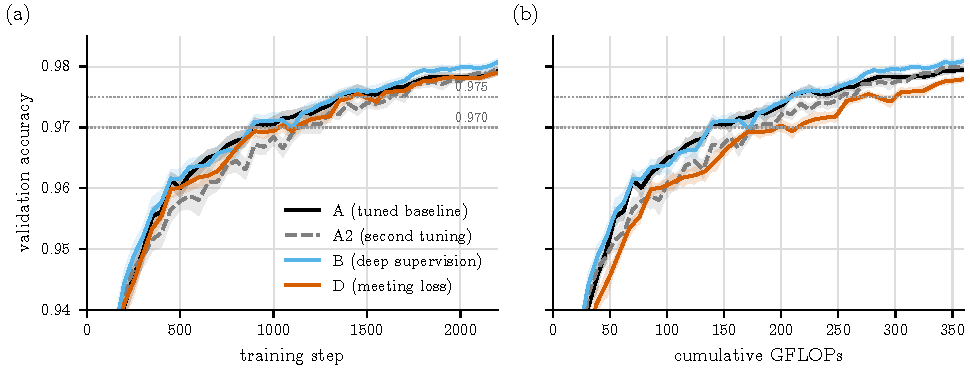
\includegraphics[width=\textwidth]{fig_s1_curves}
\caption{Study 1: validation accuracy against (a) training steps and (b) cumulative GFLOPs, mean of 20 seeds with $95\%$ bands. Dotted lines: the two targets. Arm D (orange) is below the baseline in both panels; B (blue) overlaps A; the second tuning A2 (dashed) is slower than A. Triangles on the lower axis of the GFLOPs panel mark the mean cost to reach $0.975$ under the per-seed scoring rule.}
\label{fig:s1-curves}
\end{figure}

\paragraph{Same-cost control.} B costs only $0.6\%$ more per step than A, so it is the right control for ``any auxiliary loss'': the meeting loss did worse than the same-cost control \emph{and} than the plain baseline. At the secondary target $0.98$, which is not part of the verdict, B was ahead of A and A2 (it missed the target in 1 of 20 seeds, A in 8 and A2 in 3), which is recorded as a lead and not as a claim.

\section{Controls and variants}\label{sec:desc}
Seven further groups were run on 10 seeds as descriptive groups that decide no claim (\cref{tab:s1-desc} and \cref{fig:s1-forest}). They address the explanations that a null result invites. None of them reaches the baseline.
\begin{itemize}
\item \textbf{Variants of the meeting loss.} Noise in the inverse loss (V1) costs $48.5\%$ and $55.0\%$ more, more than its per-step overhead ($+34.6\%$) alone, so it also needs more steps. The augmented output (V2) costs $45.3\%$ and $44.5\%$ more, which is almost exactly its per-step overhead ($+44.6\%$): it needs about the same number of steps as A. The frozen random inverse V3, the cheapest variant ($+11.7\%$ per step), is $+8.6\%$ and $+22.4\%$ and so shows no gain either.
\item \textbf{Controls.} Deep supervision with the reference-code schedule (B-code) is level with A. Neither the exact-gradient target (F, $+27.7\%$ and $+19.9\%$) nor the lower-layer learning-rate multiplier (E, $+40.2\%$ and $+30.0\%$) helps, so the absence of a gain is not the result of a lower-layer step-size effect that the tuned baseline failed to exploit. The autoencoder auxiliary (C) costs more than twice as much as A.
\end{itemize}
These tests show that the null result is not specific to one detail of the loss, but they do not exclude every possible variant.

\begin{table}[t]
\centering\small
\caption{Study 1, descriptive groups (10 seeds, paired with seeds 0--9 of A). Paired percentage change of mean FLOPs-to-target against A with $97.5\%$ bootstrap intervals. No group is cheaper than A.}
\label{tab:s1-desc}
\begin{tabular}{@{}l l l@{}}
\toprule
Group & to 0.97 & to 0.975\\
\midrule
V3 frozen random $G$ & $+8.6$ [$-2.9$, $+17.0$] & $+22.4$ [$+12.1$, $+37.5$] \\
V2 augmented output & $+45.3$ [$+32.6$, $+60.4$] & $+44.5$ [$+31.4$, $+61.9$] \\
V1 noisy inverse & $+48.5$ [$+33.2$, $+65.6$] & $+55.0$ [$+37.3$, $+74.6$] \\
F exact-gradient target (control) & $+27.7$ [$+13.0$, $+41.9$] & $+19.9$ [$+6.6$, $+36.6$] \\
E lower-layer lr multiplier (control) & $+40.2$ [$+25.3$, $+56.1$] & $+30.0$ [$+18.1$, $+43.5$] \\
B-code (DSN reference-code variant) & $+3.9$ [$-7.8$, $+14.9$] & $+2.9$ [$-8.0$, $+18.6$] \\
C autoencoder auxiliary & $+135.6$ [$+109.1$, $+165.1$] & $+134.8$ [$+105.8$, $+165.4$]
\\
\bottomrule
\end{tabular}
\end{table}

\begin{figure}[t]
\centering
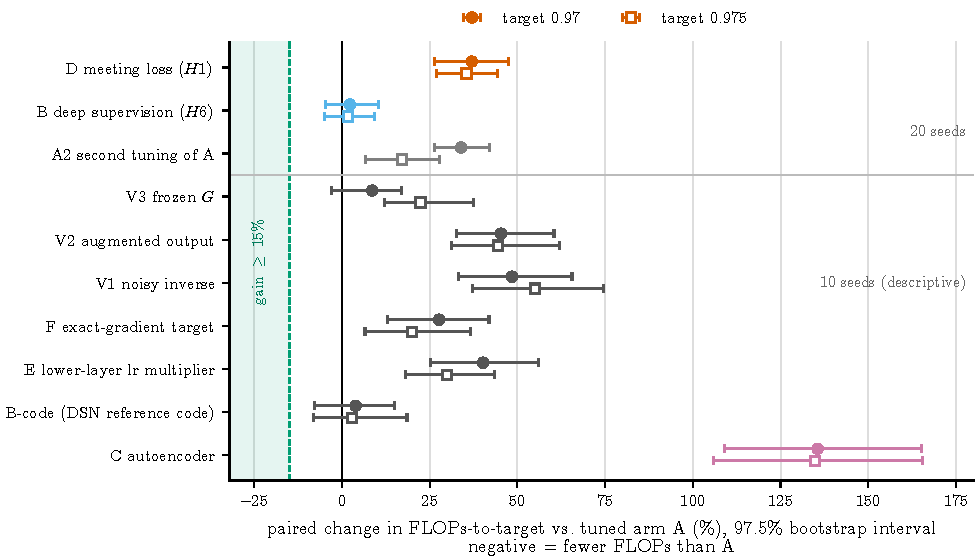
\includegraphics[width=0.92\textwidth]{fig_s1_forest}
\caption{Paired change in FLOPs-to-target against the tuned baseline A for every group of Study 1 (filled markers: target $0.97$; open: target $0.975$; $97.5\%$ bootstrap intervals). The green region is a saving of $15\%$ or more, the margin of the pre-registered hypotheses. The meeting loss (orange) and all its variants and controls are to the right of zero. Deep supervision (B) lies on zero. The second tuning of the baseline (A2) is $+34\%$ and $+17\%$.}
\label{fig:s1-forest}
\end{figure}

\section{Gradient alignment (H3)}\label{sec:h3}
A natural worry is that the meeting loss fails because its direction is simply wrong. H3 was a mechanism check: the cosine between the gradient of $\Ltask$ and that of $\Lmeet$ with respect to the lower-layer parameters, measured on the same batch during training. It was positive at $100\%$ of the evaluations and the median alignment was between $+0.75$ and $+0.79$ in every run of arm D. The direction is therefore consistent with the true gradient. High alignment together with no gain is what one would expect if the meeting signal adds little to backpropagation, which is investigated in \cref{ch:mechanism}; it is an interpretation, not a tested mechanism.

\section{A by-product: tuning on two seeds is unreliable}\label{sec:noise}
The Study 1 data contain a second result, which concerns the protocol and not the loss. The two independent tunings of the baseline tied at selection (both $232.6$ GFLOPs to $0.975$), but on 20 fresh seeds A2 needed $+34.0\%$ ($[+26.5,+42.0]$) more FLOPs than A1 to reach $0.97$ and $+17.2\%$ ($[+6.7,+27.7]$) more to reach $0.975$. The selection score of an arm overstated or understated its final value in both directions (\cref{fig:tuning-noise}a): A improved from $232.6$ to $212.4$, A2 worsened from $232.6$ to $248.9$, B worsened from $191.2$ to $216.1$ and D from $276.3$ to $287.8$. The apparent lead of deep supervision at selection ($-18\%$) vanished on fresh seeds against A ($+1.7\%$), although against A2 it is large ($-13.2\%$ to $-23.7\%$, \cref{tab:s1-vs-a2}): \emph{which} tuned baseline is used decides whether B looks better. The meeting-loss result does not depend on this choice (\cref{tab:s1-main,tab:s1-vs-a2}): D is worse than A and not better than A2.

\begin{table}[t]
\centering\small
\caption{Exploratory comparison of D and B against the second tuning A2 (20 seeds, $97.5\%$ intervals). Against A2, B looks clearly better and D is not worse at $0.97$; against A1 (\cref{tab:s1-main}) B is level and D is worse. The reference baseline therefore has to be fixed in advance.}
\label{tab:s1-vs-a2}
\begin{tabular}{@{}l l l@{}}
\toprule
Arm & to 0.97 & to 0.975\\
\midrule
D (meeting loss) & $+2.2$ $[-4.7, +9.9]$ & $+15.6$ $[+9.5, +22.5]$ \\
B (deep supervision) & $-23.7$ $[-27.8, -19.1]$ & $-13.2$ $[-18.7, -7.2]$
\\
\bottomrule
\end{tabular}
\end{table}

The across-seed variation of a \emph{fixed} configuration is small (the standard deviation of the logarithm of steps-to-$0.975$ is only $0.08$--$0.12$ on the final runs); the dominant noise is in \emph{which configuration the two-seed selection among 25 trials picks}, because the minimum of a noisy score is chosen. \Cref{fig:tuning-noise}b shows this for the Study~2 seeds with all six tunings of the baseline (\cref{sec:retune}).

\begin{figure}[t]
\centering
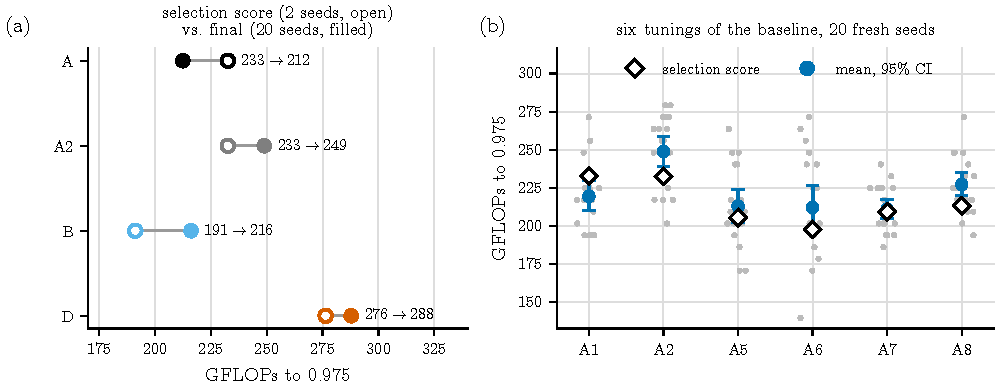
\includegraphics[width=\textwidth]{fig_tuning_noise}
\caption{Selection-stage scores are optimistic and unreliable. (a) For four arms of Study 1, the selection score on 2 seeds (open) and the mean over 20 final seeds (filled): the two tunings of the baseline tie at selection but end up $36.5$ GFLOPs apart. (b) Six independent tunings of the baseline evaluated on the 20 fresh seeds of Study 2: individual seeds (grey), mean with $95\%$ bootstrap interval (blue) and the selection score (diamond).}
\label{fig:tuning-noise}
\end{figure}

\section{Summary of Study 1}
Under a protocol that counts every FLOP, tunes every arm equally and fixes the decision rule in advance, the meeting loss did not reduce the cost of reaching $0.97$ or $0.975$ validation accuracy for this network. It needed about a third more FLOPs than the tuned baseline, because it increased the cost per step by $23\%$ and did not reduce the number of steps. No variant or control changed this. The direction of the signal is aligned with the gradient. The result is conditional on one network, one dataset, one optimiser (AdamW) and the tuned configurations; the scope is stated in \cref{sec:limitations}.
